\documentclass[12pt, titlepage]{article}
\usepackage{xcolor} % for different colour comments

%% Comments
\newif\ifcomments\commentstrue

\ifcomments
\newcommand{\authornote}[3]{\textcolor{#1}{[#3 ---#2]}}
\newcommand{\todo}[1]{\textcolor{red}{[TODO: #1]}}
\else
\newcommand{\authornote}[3]{}
\newcommand{\todo}[1]{}
\fi

\newcommand{\wss}[1]{\authornote{magenta}{SS}{#1}}
\newcommand{\ds}[1]{\authornote{blue}{DS}{#1}}

%% Graphics
\usepackage{float}
\usepackage{caption}
\usepackage{graphicx}
\usepackage{courier}
\graphicspath{ {images/} }

\begin{document}

\title{Smart Waiter Test Report} 
\author{Meraj Patel \#1137491 \\ Pavneet Jauhal \#1149311\\ Shan Perera \#1150394}
\date{\today}
\maketitle

\tableofcontents 

\listoftables

\begin{table}[H]
\section*{Revision History}
\begin{tabular}{|c|c|}
\hline
\textbf{Date}  & \textbf{Comments} \\ \hline
March 20, 2016 & Test results added \\
\hline
March 20, 2016 & Account Tests added \\
\hline
March 21, 2016 & Order Transactions added \\
\hline
March 21, 2016 & Introduction Created \\
\hline
\end{tabular}
\caption{Revision History Table}
\end{table}

\section{Introduction}
\subsection{Purpose of the Report}
This section will provide an introduction and general outline of the Smart-Waiter test report. 

\subsection{Scope of Testing}
The test report primarily focuses on the overall correctness of the software with regard to the test cases provided. Many of the test cases provided are in the form of functional dynamic tests. Automatic testing for modules in Smart-Waiter were not feasible, as mentioned in the Test Plan. This plan is fairly exhaustive, further testing will be performed for the final revision to ensure a completely smooth and intuitive user experience.

\subsection{Organization}
In section 1 we provide the introduction to the test report. In section 2 we outline and provide the results of the system testing, including but not limited to: Database security testing, order transactions testing, account testing. Section 3 describes the Usability tests that were conducted and carried out by the Smart-Waiter team.
 
\section{System Testing} 


\subsection{Database Testing}

\subsubsection{Purpose}
Database testing is critical component in correlation with Smart Waiter application. Testing was conducted to ensure users are able to retrieve and send information regarding restaurant orders.

\subsubsection{Structural Test}
Database testing was exclusively performed from structural testing point of view. The goal of this component of testing was to verify that the database queries always return valid and correct data, under all circumstances. Specifically, a separate database was created for testing purposes, because any failed test case could affect the state of the original database.\\\\
\emph{Note: A mix of scripts and manual commands were required for database testing. The tests cannot be fully automated because it is not feasible, as mentioned in test plan.}
\subsubsection{Test Factors}
As per test plan, the following test factors will be considered for database testing;
\begin{itemize}
 \item Correctness
 \item Performance
 \item Security
 \item Reliability
 \end{itemize}

\subsubsection{Correctness}
In this section of database testing, tester had to verify that the application receives complete and correct data from the couchbase server.
\subsubsection{Correctness Tests Results}
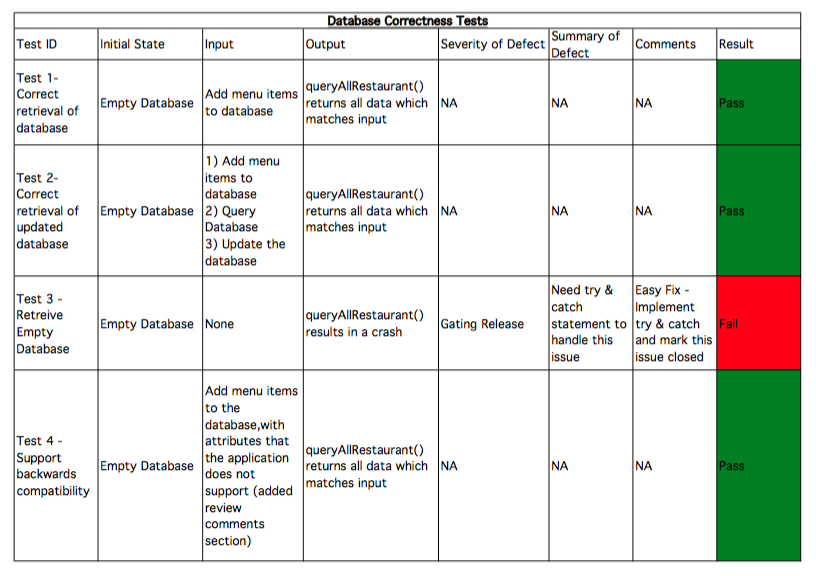
\includegraphics[width=\textwidth,height=\textheight,keepaspectratio]{correctness_tests.png}

\subsubsection{Performance}
In this section of database testing, tester had to verify that the data query was performed in a reasonable amount of time. 
\subsubsection{Performance Test Results}
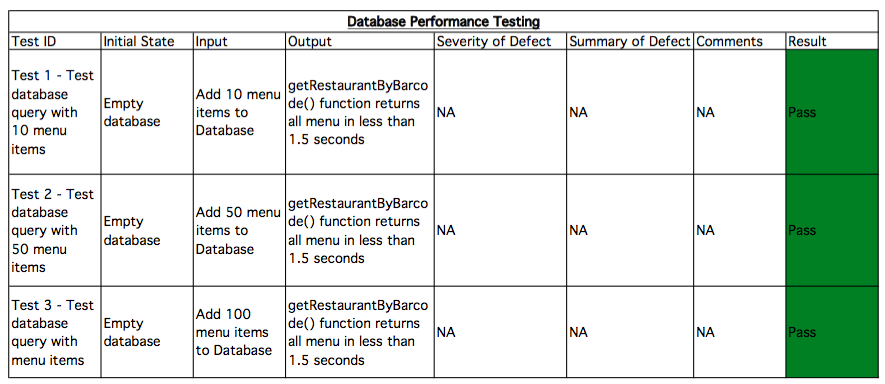
\includegraphics[width=\textwidth,height=\textheight,keepaspectratio]{performance_tests.png}

\subsubsection{Security}
In this section of database query testing, tester had to verify that database allows correct access control. Database penetration testing was not required because we will leverage couchbase security implementation, testing and certifications.
\subsubsection{Security Test Results}
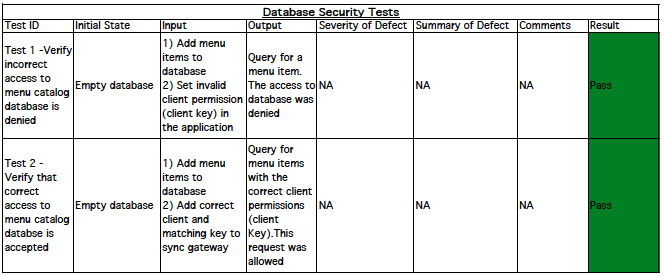
\includegraphics[width=\textwidth,height=\textheight,keepaspectratio]{security_tests.png}

\subsubsection{Reliability}
In this section of database testing, we tested the robustness and reliability of the database. 
\subsubsection{Reliability Automated Test Results }
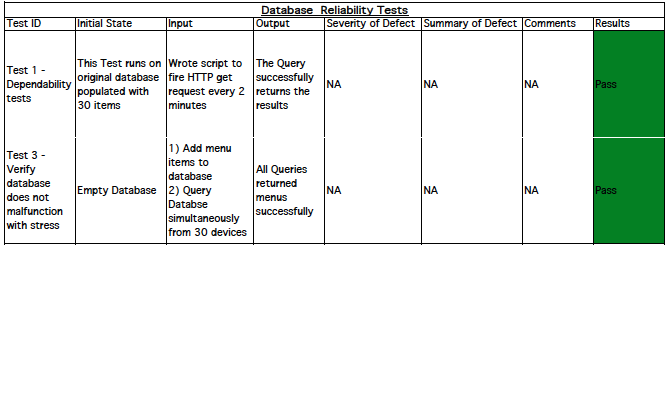
\includegraphics[width=\textwidth,height=\textheight,keepaspectratio]{reliability_tests.png}


\subsection{Barcode Scanning}

\subsubsection{Purpose}
Barcode scanning tests were conducted to make sure users are able to scan a barcode with minimal attempts. Also, to check if appropriate messages are displayed according to each test case.

\subsubsection{Test Factors}
\begin{itemize}
 \item Correctness
 \item Performance
 \item Ease of use
 \end{itemize}

\subsubsection{Correctness, Performance and Ease of use}
Testing is performed to ensure barcode scanning provides correct results in an efficient and timely manner. As well to make sure user is easily able to scan the barcode and is provided helpful messages in regards to errors encountered.

\subsubsection{Functional Unit Test}
As per our test plan, functional unit tests were  conducted to assess test cases. Doing so replicates real world usage.

\subsubsection{Test Results}
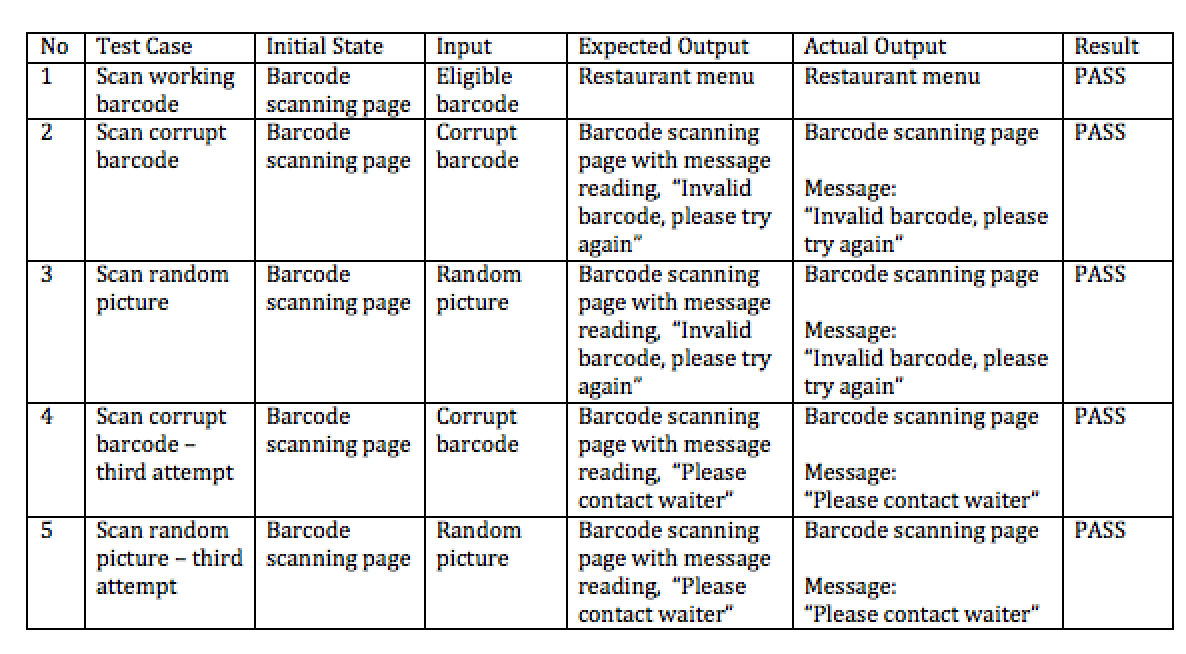
\includegraphics[width=1.2\textwidth]{barcodeTable.png}

\subsection{Accounts}
\subsubsection{Purpose}
Account creation and login tests were performed to ensure Smart-Waiter users are able to create an account quickly while still adhering to the account constraints set by Smart-Waiter. This is also to ensure proper error checking is implemented in the applications account related modules.
\subsubsection{Functional Dynamic Test}
As per our test plan, manual functional dynamic tests we performed to assess the following test cases. This allows the system to be exhaustively tested which will minimize or completely erase errors in real world usage.
\subsubsection{Test Factors}
As per test plan, the following test factors will be considered for database testing;
\begin{itemize}
 \item Correctness
 \item Data Integrity
 \end{itemize}
\subsubsection{Correctness and Data Integrity}
In this section of Account testing, the tester had to verify that all data being passed is in the correct format and that the passwords were being stored properly so that user logins can be authenticated. 

\subsubsection{Test Results}
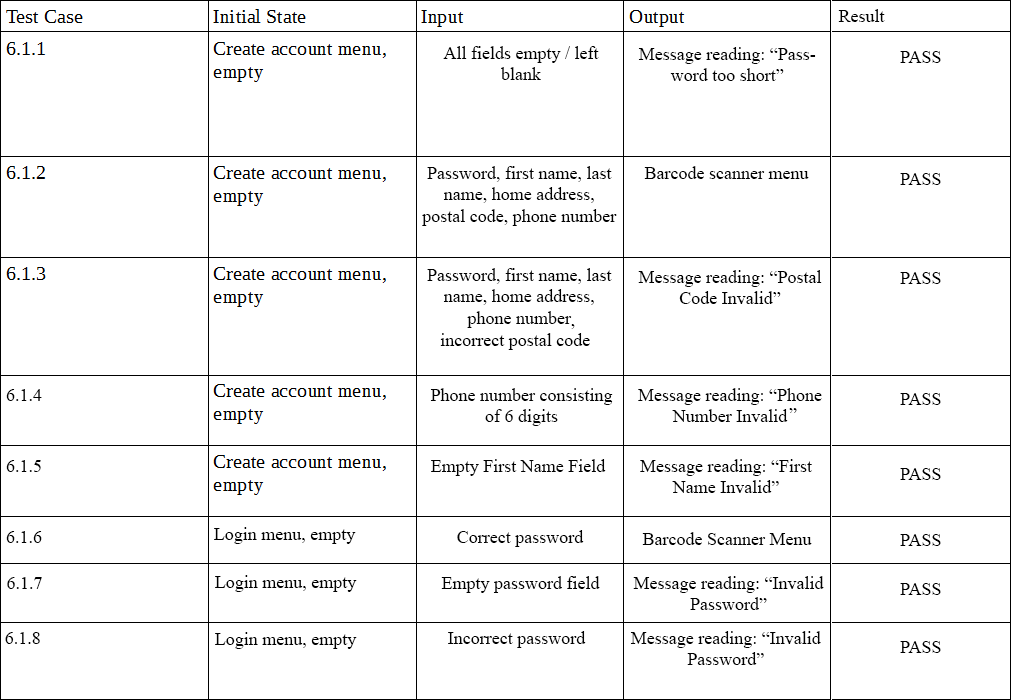
\includegraphics[width=1.2\textwidth]{accountTC.png}

\subsection{Order Transactions}

\subsubsection{Purpose}
Order transactions are a critical part of Smart-Waiter, any unforeseen bugs or errors could effect the operations of the restaurant. Therefore, these modules of Smart-Waiter were rigorously tested to ensure no unexpected behaviour and a smooth and intuitive experience. Tests were performed to ensure Smart-Waiter users are able to order from the restaurants menu quickly without having to wait for a server to arrive. This is also to ensure proper error checking is implemented in the applications transaction related modules.

\subsubsection{Functional Dynamic Test}
As per our test plan, manual functional dynamic tests we performed to assess the following test cases. In a few of these test cases, manual testing for unexpected behaviour was performed by passing unexpected input. This is so any unexpected errors that may come up from unusual input is identified and fixed so that this does not add any extra work or effect the day-to-day operations of our restaurant partners. The two test cases that are performed to identify any unexpected behaviour is 6.2.1 and 6.2.7 in the table below. The 6.2.1 test is performed by rapidly clicking different sides that are available in the sides menu before the application transitions to the next activity. The 6.2.7 test is performed by selecting toppings for an entree menu item. Then editing the toppings using the function available in the order summary page, the toppings are changed and the side is changed and added to cart multiple times. These tests yielded no strange behaviour, and the application performed as expected. 


\subsubsection{Test Factors}
As per test plan, the following test factors will be considered for database testing;
\begin{itemize}
 \item Correctness
 \item Reliability
 \item Data Integrity
 \end{itemize}
\subsubsection{Correctness, Reliability and Data Integrity}
In this section of Order Transaction testing, the tester had to verify that all data being passed is in the correct format and valid. Multiple tests to verify that the credit card information being passed is valid are performed. The tests are also used to check the reliability of the Stripe API and overall error testing. Some test cases check for unexpected behaviour in the Sides and Toppings module of the application by performing unexpected input. This is done to test the overall reliability of the Orders module.    

\subsubsection{Test Results}
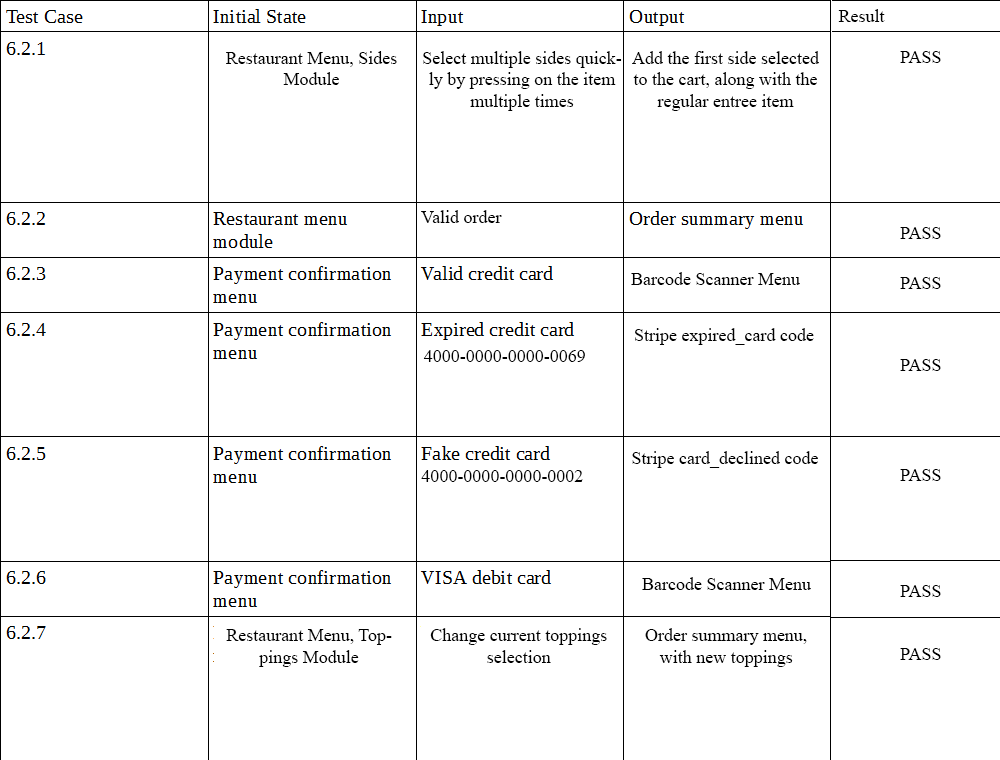
\includegraphics[width=1.2\textwidth]{orderTransactionTC.png}

\section{Usability Test}
Usability tests are conducted to assess the user's ability to complete routine tasks, and acquire their impression of the application.
\subsection{Summary}

To retrieve insightful results, participants were asked to complete a series of tasks and answer a brief questionnaire afterwards. 
\\\\
The first usability test has already been conducted on February 4, 2016. A total of six participants were gathered to conduct this test. To replicate an adequate demographic, three participants chosen are experienced using android applications, while the remaining three have little to no experience. 
\\\\
The proceeding sections provide insight and results of the usability test conducted. 

\subsection{Methodology}

\subsubsection{Tasks conducted}
Participants were given a list of tasks to complete including: 
\begin{itemize}  
\item Task 1: Create and login to account
\item Task 2: Scan barcode to retrieve menu
\item Task 3: Customize and add items to cart
\item Task 4: View cart
\item Task 5: Delete item
\item Task 6: Modify item
\item Task 7: Confirm and pay for order
\end{itemize}
\subsubsection{Questionnaire}
Participants were asked to rate from 1 to 5 (1 - strongly disagree, 5 - strongly agree), provided the following statements: 
\begin{enumerate}
\item  I was able to complete the task quickly using the system
\item It was easy to learn how to use the system
\item I prefer using Smart-Waiter over ordering in a traditional sense
\item The interface of the system was pleasant
\item The system has all the functions and capabilities I expect it to have
\item Whenever I made a mistake using the system, I could recover easily and quickly
\item Overall I was happy using the system
\end{enumerate} 

\subsection{Testing Results} 

\subsubsection{Questionnaire Results}

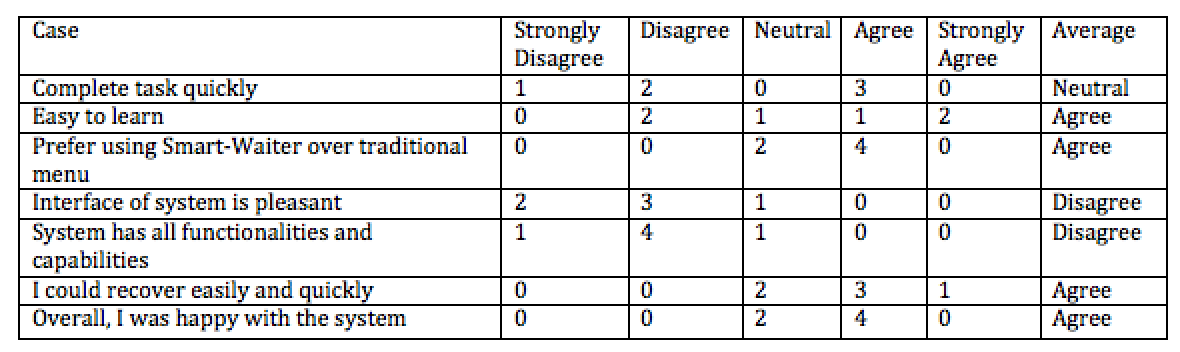
\includegraphics[width=1.2\textwidth]{usabilityResults.png}

\subsubsection{User Feedback}

After completing the usability test, we asked participants for feedback in terms of their experience. Specifically we asked for their; likes, dislikes and recommendations. 
\\\\
\textbf{Likes} 
\begin{itemize}
\item Convenient for ordering take out at restaurant  
\item Ability to customize items and send special instructions
\item Ease of use (according to experienced android application users)
\end{itemize}
\textbf{Dislikes}
\begin{itemize}
\item Look of GUI
\item Unable to modify account settings
\item Unable to save receipt 
\end{itemize}
\textbf{Recommendations}  
\begin{itemize}
\item Add settings page
\item Offer ability to email receipt
\end{itemize}
\subsection{Conclusion}
Conducting this usability test definitely helps our team in terms of adjusting requirements to meet user recommendations. Specifically the following changes will be implemented: 
\begin{itemize}
\item Create settings page
\item Improve GUI
\item Allow users to view order history
\end{itemize}
After implementation of these additions, a second usability test will be conducted. New participants will be gathered in order to provide unbiased results. 
\end{document}